\documentclass[12pt, letterpaper]{article}
\usepackage[utf8]{inputenc}
\usepackage[margin=2cm]{geometry}
\usepackage{amsmath}
\usepackage{amssymb}
\usepackage{graphicx}
\usepackage{cancel}
\usepackage{fancyhdr}
\usepackage{float}
\usepackage{mwe,tikz}\usepackage[percent]{overpic}

\graphicspath{ {./bilder/} }

\title{ \begin{huge}
\textbf{Portfolio Assignment 3}
\end{huge} }

\author{Candidate 25}
\date{}

\rfoot{\thepage}
\newcommand{\bs}{\boldsymbol}
\newcommand{\mbf}{\mathbf}

\begin{document}
\maketitle
  \section*{Problem 1}
    \subsection*{(1a)}
      I shall now discuss the main difference between feature extraction and feature selection.
    \subsection*{(1b)}
      In this problem I implemented a program which used the multidimensional scaling algorithm (MDS), to reduce the number of dimensions in the final output. The way MDS works is by using a result from linear algebra known as eigendecomposition, which uses the eigenvalues and eigenvectors to make what might have began as data structured with 10 features and many datapoints, into data with only 2 or 3 features.\\
      In this task we are interested in reducing a 34 x 34 matrix which contains the geodesic distances between 34 swedish cities, into something we can plot on a two dimensional map.\\
      To do this we use MDS and specify that we only want 2 dimensions on the resulting coordinate matrix.
    \subsection*{(1c)}
      \begin{figure}[H]
        \caption{Resulting 2 dimensional plot of 34 Swedish cities.}
        \centering
        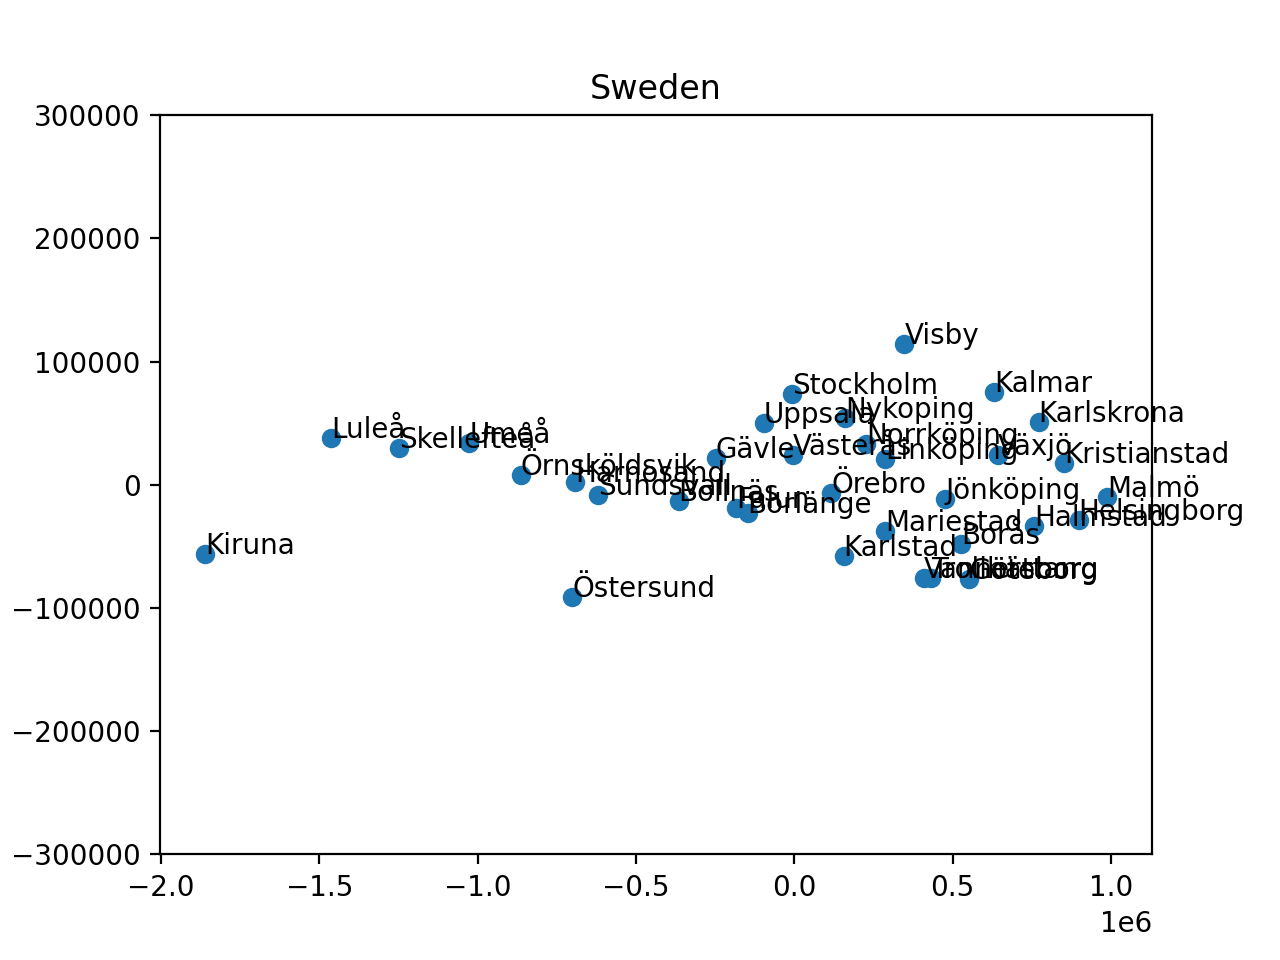
\includegraphics[scale=0.7]{Swedishcities}
        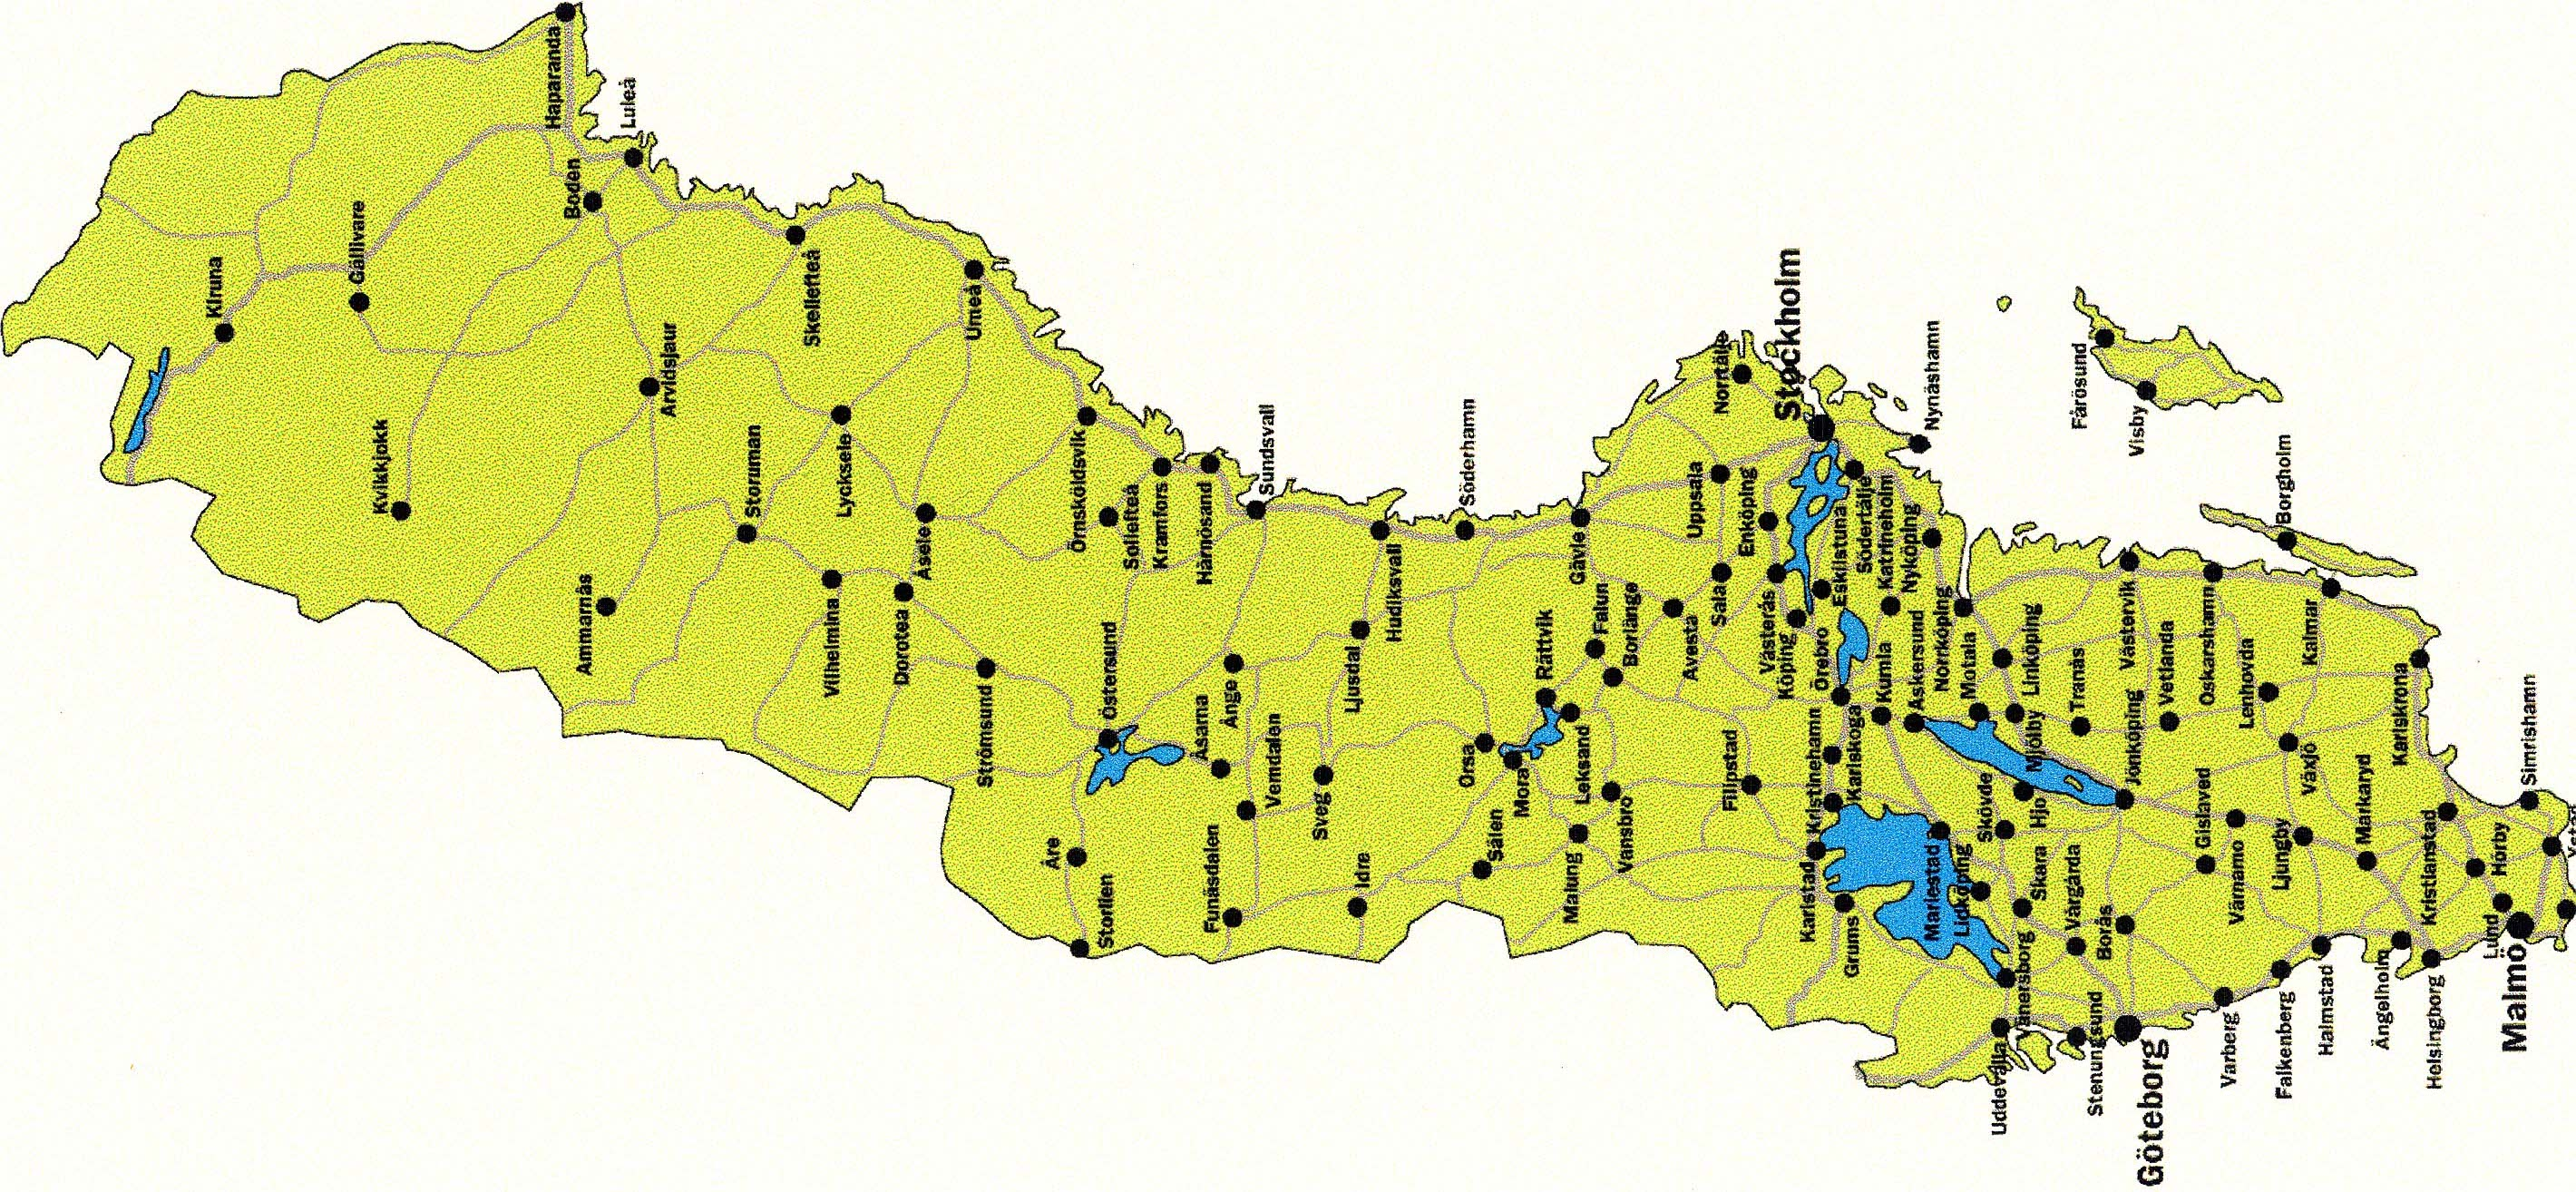
\includegraphics[scale=0.1]{Swedishmap}
      \end{figure}\\
\end{document}
